% Chapter 3
\chapter{Contributions\label{chapter:contributions}}% For referencing the chapter elsewhere, use \ref{chapter:contributions} } % Main chapter title

In this chapter, we introduce our RGTDSMF methodology. We will describe our new weighting scheme and our novel windowing technique for ensembles. We will then cover our improvement to the voting classifier to reduce the dependency on ground truth during training. Next, we will explain how we extended FHDDM and FHDDMS to work without ground truth. Finally, we will cover all of our contributions by using a small toy example to explain how data is processed from a stream.

%----------------------------------------------------------------------------------------

\section{Voting Classifier: Weighting and Voting Schemes \label{section:new_voting_strategy}}

The reader may refer to section \ref{section:new_voting_strategy} for background on ensembles and voting classifiers.

A voting classifier was extracted from the mlxtend library\footnote{\url{http://rasbt.github.io/mlxtend/user_guide/classifier/EnsembleVoteClassifier/}}, developed by Sebastian Raschka. Mlxtend is an extension of the scikit-learn python machine learning library, to handle classification in a streaming setting.

The mlxtend voting classifier implements two voting strategies: the first being "soft" voting and the second being "hard" (majority) voting; again, refer to section \ref{section:new_voting_strategy} for their definitions.

We implemented two additional voting schemes similar to the "soft" scheme in that they require its classifiers to output a probability or confidence in the class label prediction. The first method makes use of a logistic function with a sigmoid curve to weigh the probability, centered around a  confidence level. Let $\alpha$ be the parameter that defines the confidence level, set to \textbf{\textit{$\alpha=50\%$}}. And the second method, explained soon thereafter is equivalent to the function of the first method while being less computationally intensive.


Logistic functions are defined by the function in equation \ref{eq:logistic_function}
\begin{equation}
    f(x)=\frac{L}{1+e^{-k(x-x_0)}}\\ 
    \label{eq:logistic_function}
\end{equation}
where \textit{e} is the natural logarithm base, \textit{$x_0$} is the x-value of the sigmoid's midpoint, \textit{L} is the curve's maximum value, and \textit{k} is the steepness of the curve.

The logistic function that we initially selected had the following values for the variables listed above. $x_0=0.65$, $L=1$, and $k=14$. These values were selected based on the resulting graph for values of $x \in [0, 1]$ and $f(x) \in [0, 1]$. As you can see from figure \ref{graph:weights}, predictions with less than approximately forty percent probability are essentially treated as predictions with zero probability; predictions with under a seventy percent probability are diminished in importance, and those over seventy percent are boosted. Refer to table \ref{table:weight_probabilities} to see how the values change by five and ten percent increments. The reasoning motivating this choice is our intuition that we should put more trust in predictions with over seventy percent (70\%) probability, put less trust in predictions with a probability of under seventy percent  (70\%), and virtually none in predictions with a probability under forty percent (40\%).

\begin{figure}
  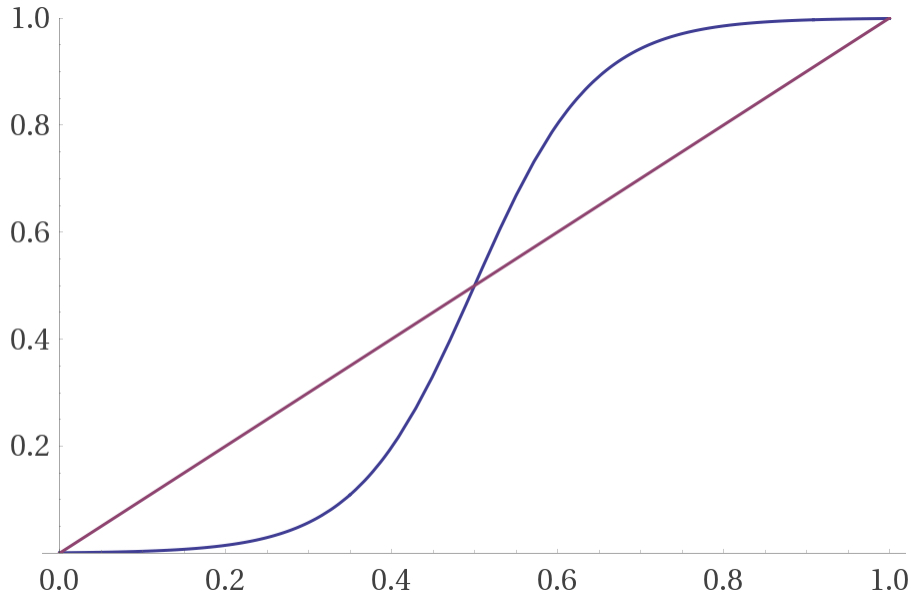
\includegraphics[width=\linewidth]{./images/weight_graph}
\caption{\label{graph:weights}Voting classifier weighting functions\\\protect\blueline$x$\\
\protect\redline $\frac{1-tanh(3.5-7x)}{2}$}
\end{figure}

However, after extensive experimentation, of which the results are found in tables \ref{table:weighting_experimental_test} and \ref{table:weighting_experimental_test_all_datasets}, we found that setting \textbf{$x_0=0.50$} and \textbf{$k=14$} was more optimal than the values we initially selected through intuition for the $x_0$ and $k$ parameters.

The same test as above was repeated, but, over four separate datasets for the two best combination of parameters and the one from our intuition ($k=14$, and $x_0 \in [0.5, 0.55, 0.65]$), and ran only once. Table \ref{table:weighting_experimental_test_all_datasets} shows, again, that $k=14, x_0=0.50$ seems to be the optimal set of parameters as it obtains the best results for three out of four datasets.

\begin{table}[]
\caption{\label{table:weighting_experimental_test}Experimental test of weighting function parameters}
\centering
\begin{tabular}{|c|c|c|c|c|}
\hline
\textbf{Parameters} & \textbf{Accuracy} & \textbf{$\kappa$} & \textbf{$\kappa_t$} & \textbf{$\kappa_m$} \\ \hhline{=====}
\textit{no weighting}&81.95&61.47&61.10&52.78 \\ \hline
10, 0.65&83.56&64.77&64.57&57.00 \\ \hline
14, 0.45&84.28&66.26&66.12&58.88 \\ \hline
\textbf{14, 0.50}&\textbf{84.77}&\textbf{67.34}&\textbf{67.17}&\textbf{60.15} \\ \hline
\textbf{14, 0.55}&\textbf{84.72}&\textbf{67.25}&\textbf{67.06}&\textbf{60.02} \\ \hline
14, 0.65&83.75&65.12&64.98&57.49 \\ \hline
14, 0.6&84.22&66.13&65.98&58.71 \\ \hline
14, 0.75&81.73&60.86&60.63&52.21 \\ \hline
14, 0.85&80.51&58.65&57.99&49.01 \\ \hline
5, 0.65&82.77&63.03&62.85&54.91 \\ \hline
7, 0.65&83.04&63.56&63.44&55.62 \\ \hline
\end{tabular}
\end{table}

\begin{table}
\caption{\label{table:weighting_experimental_test_all_datasets}Experimental test of weighting function parameters on 4 datasets}
\centering
\begin{tabular}{|c|c|c|c|c|c|}
\hline
\textbf{Dataset} & \textbf{Parameters} ($k=14$) & \textbf{Accuracy} & \textbf{$\kappa$} & \textbf{$\kappa_t$} & \textbf{$\kappa_m$} \\ \hhline{======}
& $x_0=0.5$	&	84.30	&	68.60	&	68.69	&	68.73\\ \cline{2-6}
sine1 & $x_0=0.55$	&	84.15	&	68.30	&	68.39	&	68.44\\ \cline{2-6}
 & $x_0=0.65$	&	83.79	&	67.59	&	67.67	&	67.72\\ \hhline{======}
 & $x_0=0.5$	&	79.95	&	59.90	&	60.07	&	60.12\\ \cline{2-6}
mixed & $x_0=0.55$	&	79.89	&	59.78	&	59.96	&	60.01\\ \cline{2-6}
 & $x_0=0.65$	&	79.60	&	59.20	&	59.38	&	59.43\\ \hhline{======}
 & $x_0=0.55$	&	79.72	&	59.45	&	59.44	&	59.15\\ \cline{2-6}
circles & $x_0=0.65$	&	79.43	&	58.87	&	58.87	&	58.57\\ \cline{2-6}
 & $x_0=0.5$	&	77.72	&	55.45	&	55.45	&	55.13\\ \hhline{======}
 & $x_0=0.5$	&	85.20	&	68.27	&	68.10	&	61.28\\ \cline{2-6}
SEA & $x_0=0.55$	&	84.25	&	66.25	&	66.05	&	58.80\\ \cline{2-6}
 & $x_0=0.65$	&	83.41	&	64.38	&	64.25	&	56.60\\ \hline
\end{tabular}
\end{table}

\begin{table}[]
\caption{\label{table:weight_probabilities}Probabilities after weighting}
\centering
\begin{tabular}{|c|c|c|c|c|c|c|c|c|c|c|c|}\\ \hhline{============}
\textbf{Probability (\%)} & 0-10&20&30&40&50&60&65&70&75&80-85&90-100 \\ \hline
\textbf{Weighted (\%)} & 0&1&6&20&50&80&89&94&97&99&100 \\ \hline
\end{tabular}
\end{table}

We must note that $\forall x \in [0,1], f(x) \in [0, \frac{1}{1+e^{-7}}\approx 0.9991]$ for the function in equation \ref{eq:logistic_function} , we could then divide the function by its value for the maximum value for $p_i(X)$ (which is 1) to ensure that our function covers all values in $[0,1]$, but this is unnecessary as all values will be be in the same range, and it adds another calculation.
Refer to figure \ref{graph:weights} for the plot of equation \ref{eq:logistic_function_params}.

\begin{equation}
\frac{1}{1+e^{-14(p_i(X)-0.50)}}
\label{eq:logistic_function_params}
\end{equation}

Our proposed voting strategy therefore computes the average of this logistic function using the prediction of each classifier for each class label. See the following equation:
\begin{equation}
\frac{1}{n}\sum_{i=1}^{n}\frac{1}{1+e^{-14(p_i(X)-0.50)}}\\ 
    \label{eq:logistic_sum}
\end{equation}
where $n$ is the number of classifiers in the voting ensemble, and $p_i(X)$ is the probability of classifier $i$ predicting that the tuple in question belongs to class X.

We propose another weighting equation to determine if it is possible to achieve similar results by using a different function that resembles the logistic sigmoid function presented above while being less computationally intensive. As Dr. LeCun states in \citep[10]{lecun2012efficient},  "hyperbolic tangent functions often converge faster than the standard logistic function".
Our hyperbolic tangent weighting function is seen in equation \ref{eq:tanh_weight_fn} and the sum is seen in equation \ref{eq:tanh_sum}. The plot of equation \ref{eq:tanh_weight_fn} is completely identical to the plot of \ref{eq:logistic_function}.
\begin{equation}
    f(x)=\frac{1-tanh(3.5-7x)}{2}
    \label{eq:tanh_weight_fn}
\end{equation}
\begin{equation}
\frac{1}{n}\sum_{i=1}^{n} \frac{1-tanh(3.5-7\times p_i(X))}{2}
    \label{eq:tanh_sum}
\end{equation}
The calculation of averages presented in equations \ref{eq:logistic_sum} and \ref{eq:tanh_sum} are calculated for each class label. The class label with the highest average is thereafter selected as the winner in the vote. We want to test the hypothesis that weighting the predictions by an exaggeration of their probability will increase the accuracy of our voting classifier.

In order to confirm that the new weighting function was more computationally efficient, we compared the total running time to evaluate each weighting function ten million times on a random value in [0, 1]. The benchmark showed, as seen in table \ref{table:weight_benchmark}, that the logistic function takes almost 3.5 times longer to compute than the hyperbolic tangent function, which will, therefore, be used for the remainder of this thesis.

\begin{table}[]
\centering
\caption{\label{table:weight_benchmark}Weighting function benchmark results}
\begin{tabular}{|c|c|}
\hline
\textbf{Sigmoid function} & \textbf{Hyperbolic tangent} \\ \hhline{==}
1441.05 ns/class/loop & 407.40 ns/class/loop \\ \hline
\end{tabular}
\end{table}

Algorithm \ref{alg:new_voting_scheme} shows the implementation of this new voting scheme using the hyperbolic tangent function. Figure \ref{graph:weights} shows a plot with the two new proposed weighting functions and compare them to the value of an unweighted prediction represented by $f(x) =x$, for  $x \in [0,1]$. This figure shows how much a value is boosted or reduced compared to its original value

Given that the hyperbolic tangent function selected is equivalent to the logistic sigmoid function, it is not necessary to test its parameters experimentally as they give the exact same output. Figure \ref{fig:boxplots_params} shows the boxplots of table \ref{table:weighting_experimental_test}. The whiskers correspond to the minimum and maximum values over 10 runs with each parameter. The dotted diamond corresponds to the standard deviation, the dotted line in the box corresponds to the mean, while the solid line corresponds to the median.

\begin{figure}
  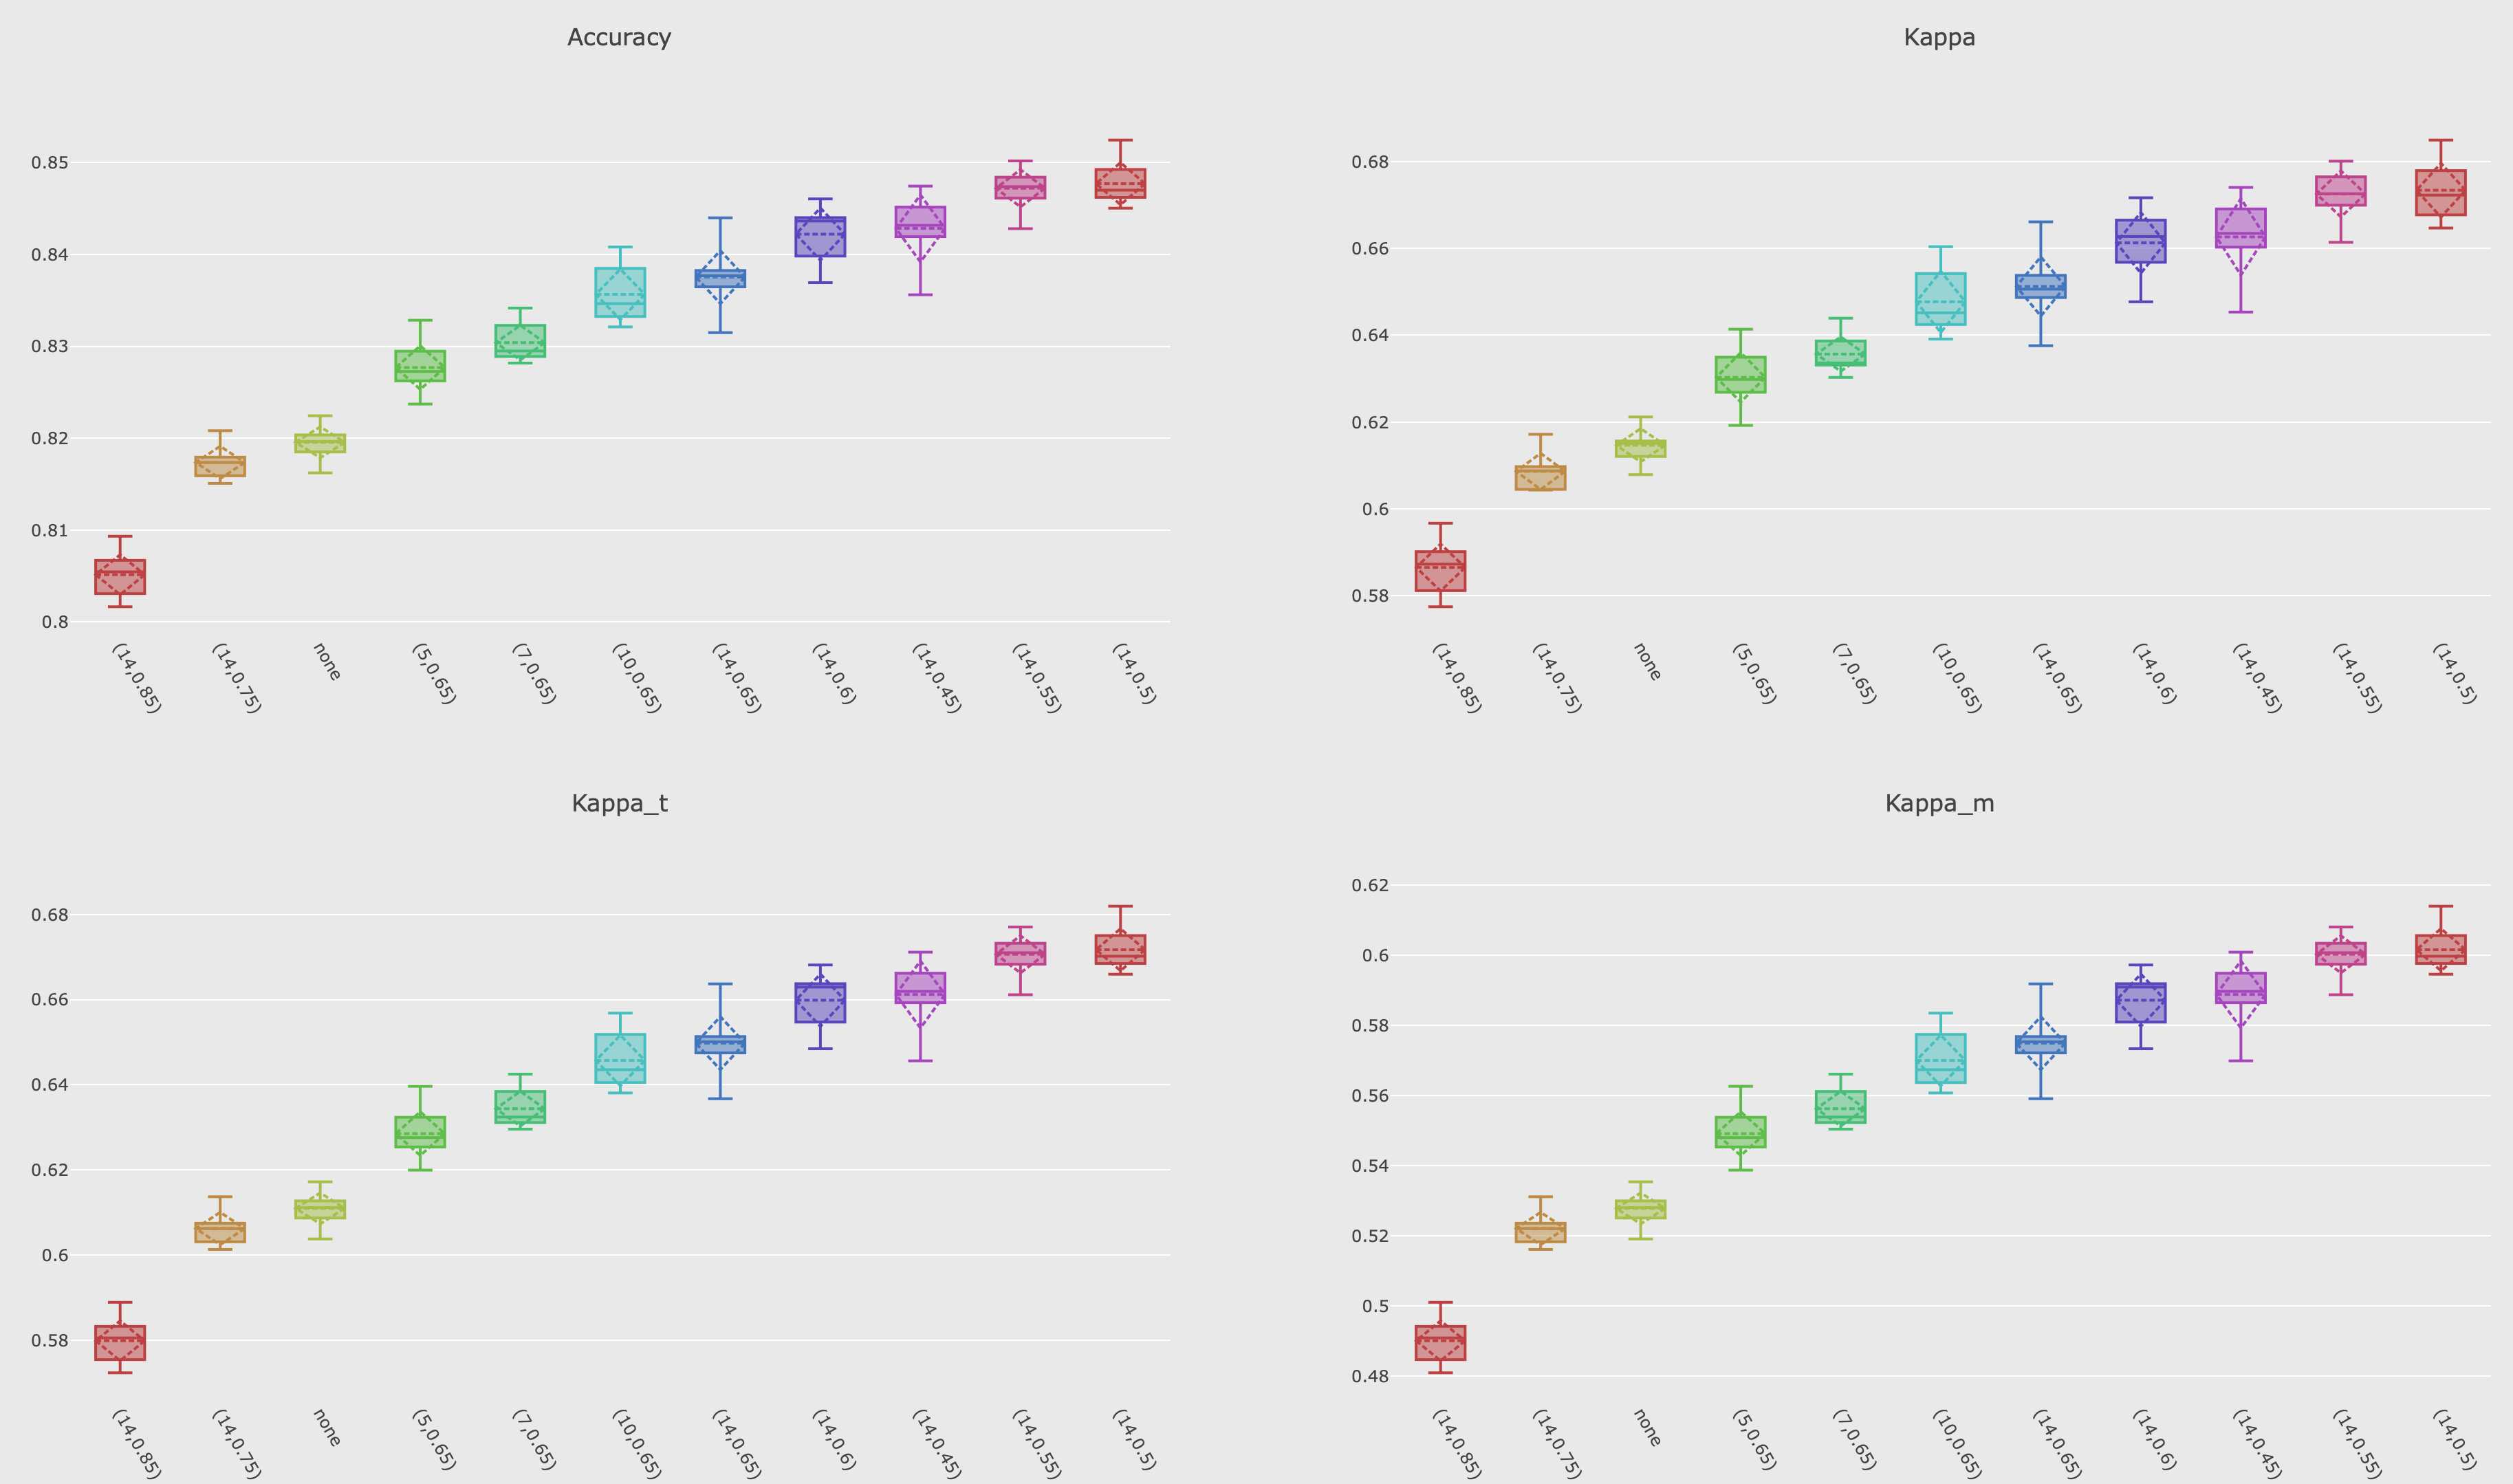
\includegraphics[width=\linewidth]{./images/boxplots_params}
\caption{\label{fig:boxplots_params}Boxplots of experimental test for logistic function parameters}
\end{figure}


\begin{algorithm}
    \caption{\label{alg:new_voting_scheme}tanh weighting scheme for voting classifier}
    \Fn{voting\_classifier.predict(X)}{
        \tcc{The probabilities are stored in a $1\times2$ matrix (using binary classification for simplicity) where each column represents a class, and each row represents a sub-classifier}
        weighted\_probabilities = []\;
        \ForEach{$classifier \in voting.classifiers$}{
            array = classifier.predict()\;
            $w\_p$ = [weight(array[0]), weight(array[1])]\;
            weighted\_probabilities.append($w\_p$)\;
        }
        \tcp{map sub-classifier probabilities to single probability}
        avg = weighted\_probabilities.avg\_over\_columns()\;
        prediction, prediction\_probability = max(avg), class\_max\_value(avg)\;
        \Return{prediction, prediction\_probability}\;
    }
    \Fn{weight(p)}{
        \Return $\frac{1-tanh(3.5-7p)}{2}$\;
    }
\end{algorithm}



%----------------------------------------------------------------------------------------

\section{Hybrid sliding-tumbling windows\label{section:hybrid-windows}}
In \cite{KRAWCZYK2017132}, B. Krawczyk mentions that one of the many issues in data stream mining is execution time, in the sense that our algorithm must learn faster than tuples can arrive. In our case, we aim to determine if we can delay training of some classifiers in our ensemble, and see how it affects execution time and classifying performance, as well as drift detection performance.

We propose the following algorithm, implemented in algorithm \ref{alg:sliding_tumbling_windows}, titled \textit{Sliding-Tumbling windows for training the ensemble}.
Let the number of tuples (single tuple or chunk) used in the interleaved test-then-train loop iterations be \textit{number\_of\_tuples}, and let \textit{number\_of\_classifiers} be the number of classifiers in the ensemble. The ensemble will have a window size of \textit{number\_of\_tuples}*\textit{number\_of\_classifiers}. At every iteration of the interleaved test-then-train loop, we will append the new tuples to the ensemble's window and train a single classifier in the ensemble on that window. For the next \textit{number\_of\_classifiers - 1} iterations, we will train the remaining \textit{number\_of\_classifiers - 1} classifiers in the ensemble. We do this so that from the point of view of the ensemble, we are training using sliding windows. But from the point of each classifier in the ensemble, we are training them using tumbling windows.

While not used for the same purpose, my colleague Sarah D'Ettore used the same sliding batches to improve CDC-Stream in her thesis \citep{d2016fine}. Figure \ref{fig:sliding_tumbling_windows}, taken from my colleagues' thesis, shows how the algorithm works for three (3) classifiers in the ensemble with a batch size of one (1) and a window size of three (3). Each classifier will only learn from the same coloured batch; meaning that at time \textit{t}, only a single classifier has enough tuples to learn from, but the others will learn at time \textit{t+1} and finally at time \textit{t+2}. Each classifier will be learning from what essentially is a tumbling window, from their point of view, just not all from the same one, or at the same time. 

To clarify the example, at time $t_1$, our ensemble will receive only one instance, add it to the sliding window and train classifier $c_1$ on the window. At time $t_2$, another instance will be added to the window and the ensemble will train classifier $c_2$ on the new window containing two tuples. At time $t_3$, the ensemble will train classifier $c_3$ on the first purple chunk (the window now has its maximum of 3 instances). At time $t_4$, $c_2$ will learn from the first blue chunk. And at time $t_5$, $c_3$ will learn from the first green chunk. This process loops indefinitely. 

The motivation for this technique is to determine if we can spend less execution time training the classifiers and to investigate how progressively delaying training of some of the classifiers in the ensemble effects concept drift detection and classification performance while also hopefully reducing execution time.

\begin{algorithm}
\KwResult{at least one classifier in the ensemble was trained}
\tcp{voting\_ensemble stores a classifier list, its count, and, the index of the current classifier to train}
\Fn{ensemble.train(X, y)}{    
        classifier\_to\_train = classifier\_list[index]\;
        index = (index + 1) modulo (number\_of\_classifiers)\;
        classifier\_to\_train.partial\_train(X, y)\;
}
\caption{Sliding-Tumbling windows for training the ensemble\label{alg:sliding_tumbling_windows}}
\end{algorithm}

\begin{figure}
  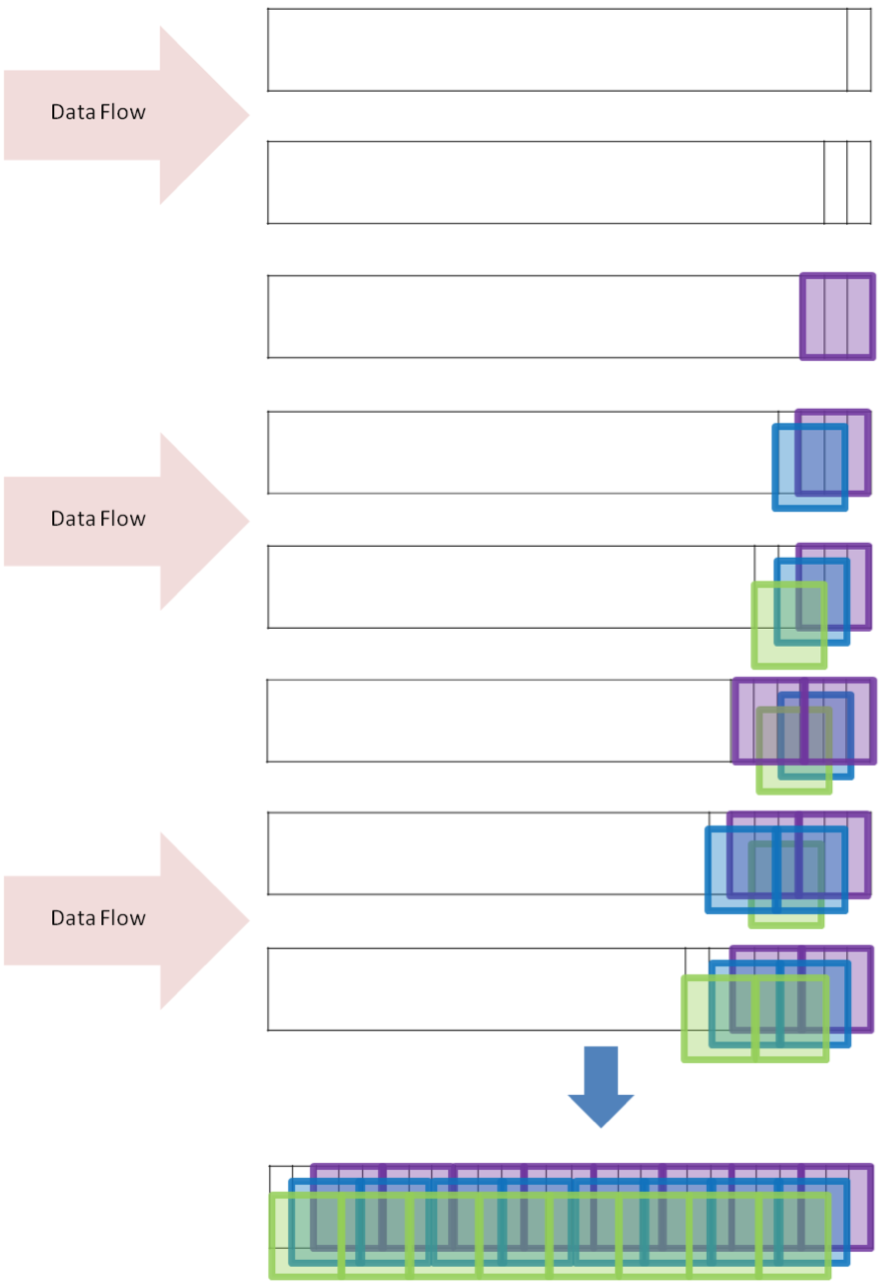
\includegraphics[width=\linewidth]{./images/sliding_tumbling_windows}
  \caption{Sliding Tumbling windows \citep{d2016fine}.}
  \label{fig:sliding_tumbling_windows}
\end{figure}



%----------------------------------------------------------------------------------------

\section{Improvements to voting classifier to reduce dependency on ground truth\label{section:vc_reduce_gt}}

The interleaved test-then-train methodology in a data streaming setting has a rather large flaw if we consider a real-life scenario: we are assuming that we obtain the ground truth immediately after testing. This means that we assume that the ground truth is always available in a fraction of a second after testing our models. For the large majority of cases, this approach is not realistic, again, in a real-world setting.

Therefore, we wanted to determine if we could re-use the idea behind self-training in an offline setting to reduce our dependency on the ground truth in the online streaming setting for the interleaved test-then-train method. We propose an approach that is, as previously stated, similar to self-training in that we use the classifier's prediction, and not ground truth, when training.

However, using only the predictions to train our model in an online setting is a recipe for disaster. The known cons to using self-training in an offline setting are that it can reinforce classification errors; it is, therefore, logical for us to come to the conclusion that we will encounter the same risks in porting this idea to a streaming setting.

Given the restriction of limiting reinforcing misclassification errors, we want to determine at what ratio of predictions to ground-truth our voting ensemble's accuracy would decline and by how much.

The algorithm behind this idea is very straightforward: it consists in duplicating the ground truth array and replacing at random a particular fraction of values with the actual prediction from the classifier, if there was no drift detected right before. See algorithm \ref{alg:self-training} to see the pseudocode (function \textit{swap ground truth with predictions}).

\begin{algorithm}
\While{stream.has\_more\_instances()}{
    X, y = stream.get\_next\_tuples(number\_of\_instances\_to\_fetch)\;
    predictions, probabilities = voting\_ensemble.predict(X)\;
    drift\_detected = voting\_ensemble.detect\_drift(predictions, probabilities)\;
    \If{$percentage \neq 100$ \textbf{and} drift not detected}{
        y = swap\_ground\_truth\_with\_predictions(y, predictions, percentage)\;
    }
 voting\_ensemble.train(X, y)\;
}

\tcp{This algorithm only shows the steps required to modify the ground truth array}
\Fn{swap\_ground\_truth\_with\_predictions(y, predictions, percentage)}{
    \For{$index=0\ \textbf{;}\ index < length(y)\ \textbf{;}\ index += 1$}{
        \If{random\_number\_between(0, 100) > percentage}{
            y[index] = predictions[index]\;
        }
    }
    \Return{y}\;
}
\caption{\label{alg:self-training}Online self-training}
\end{algorithm}

%----------------------------------------------------------------------------------------

\section{Improvements to FHDDM/S to remove dependency on ground truth: MFHDDM/S}

Additionally, this thesis builds upon my colleague's, Dr. Ali Pesaranghader, work described in section \ref{section:fhddm/s}

Along the same lines of section \ref{section:vc_reduce_gt}, the drift detection algorithm proposed by my colleague Dr. Pesaranghader in \cite{pesaranghader2016fast}, \textit{FHDDMS}, relies on the immediate knowledge of ground truth. The drift detection mechanism in FHDDMS relies on storing, in a sliding window, whether or not the classifier accurately predicted the class. This method only applies to a select few domains where ground truth can be available almost instantly after the tuples are generated, and in all synthetic data streams of course. For the large majority of domains, this method simply isn't applicable.

It is for that reason that we have set out to study if FHDDM/S is still able to detect drifts when completely removing its dependency on any knowledge of the ground truth in an online streaming setting by replacing the booleans, indicating that the classifier in/correctly predicted a class instance, stored in the sliding window by another variable.

In order to do so, we have opted to extend FHDDM and FHDDMS such that the sliding window now stores one of three values: the unweighted probability of the classifier's predicted class instance for the winning vote; the weighted probability of the classifier's predicted class instance for the winning vote; or a boolean indicating if the classifier's prediction corresponds to the ensemble's winning vote.

We implemented several approaches:
\begin{itemize}
\item one drift detector per classifier in the ensemble, storing the unweighted probabilities,
\item a single drift detector for the ensemble, storing the average of the unweighted predictions for the winning vote,
\item one drift detector per classifier in the ensemble, storing a boolean indicating if the classifier's prediction corresponds to the ensemble's winning vote.
\end{itemize}


After extensive experimentation, we were able to determine that when it comes to detecting drifts, the unweighted probabilities were no more useful than the weighted values as the difference in performance between the two is negligible. A SEA dataset was generated with 10\% noise with one-hundred thousand instances, with 4 concepts and 3 abrupt concept drifts at every twenty-five thousand instances. And the $CIRCLES$, $MIXED$ and $SINE1$ datasets were used (refer to section \ref{section:performance_measures}). When drifts were detected, all of the classifiers in the ensemble were completely reset, and one drift detector for the entire ensemble was used. In order to determine whether to use unweighted or weighted probabilities for the drift detector, we looked at the accuracy and kappa statistics of the entire stream (covered in section \ref{eq:kappa}). Table \ref{table:drift_use_weighting_experimental_test} shows these results. The values in the table are averages over 10 runs.

\begin{table}[]
\caption{\label{table:drift_use_weighting_experimental_test}Testing whether to use weighted probabilities for detecting drifts}
\centering
\begin{tabular}{|c|c|c|c|c|c|}
\hline
\textbf{Dataset} & \textbf{Weighted/Unweighted} & \textbf{Accuracy} & \textbf{$\kappa$} & \textbf{$\kappa_t$} & \textbf{$\kappa_m$} \\ \hhline{======}
SEA&\checkmark&84.53&66.77&66.66&59.53\\ \cline{2-6}
 &$\times$&84.42&66.51&66.42&59.23\\ \hhline{======}
circles&$\times$&78.35&56.71&56.70&56.39\\ \cline{2-6}
 &\checkmark&78.25&56.51&56.50&56.19\\ \hhline{======}
mixed&\checkmark&80.00&60.00&60.18&60.23\\ \cline{2-6}
 &$\times$&79.97&59.94&60.11&60.16\\ \hhline{======}
sine1&\checkmark&84.35&68.71&68.79&68.84\\ \cline{2-6}
 &$\times$&84.30&68.60&68.68&68.73\\ \hline
\end{tabular}
\end{table}

Figure \ref{fig:boxplot_params_use_w} shows the results of the experimental test from table \ref{table:drift_use_weighting_experimental_test} using boxplots. As in the table, we can see that the weighted predictions cause performance to increase ever so slightly. In the case of the $CIRCLES$ dataset, the unweighted probabilities seem to perform better than the weighted ones.

\begin{figure}
  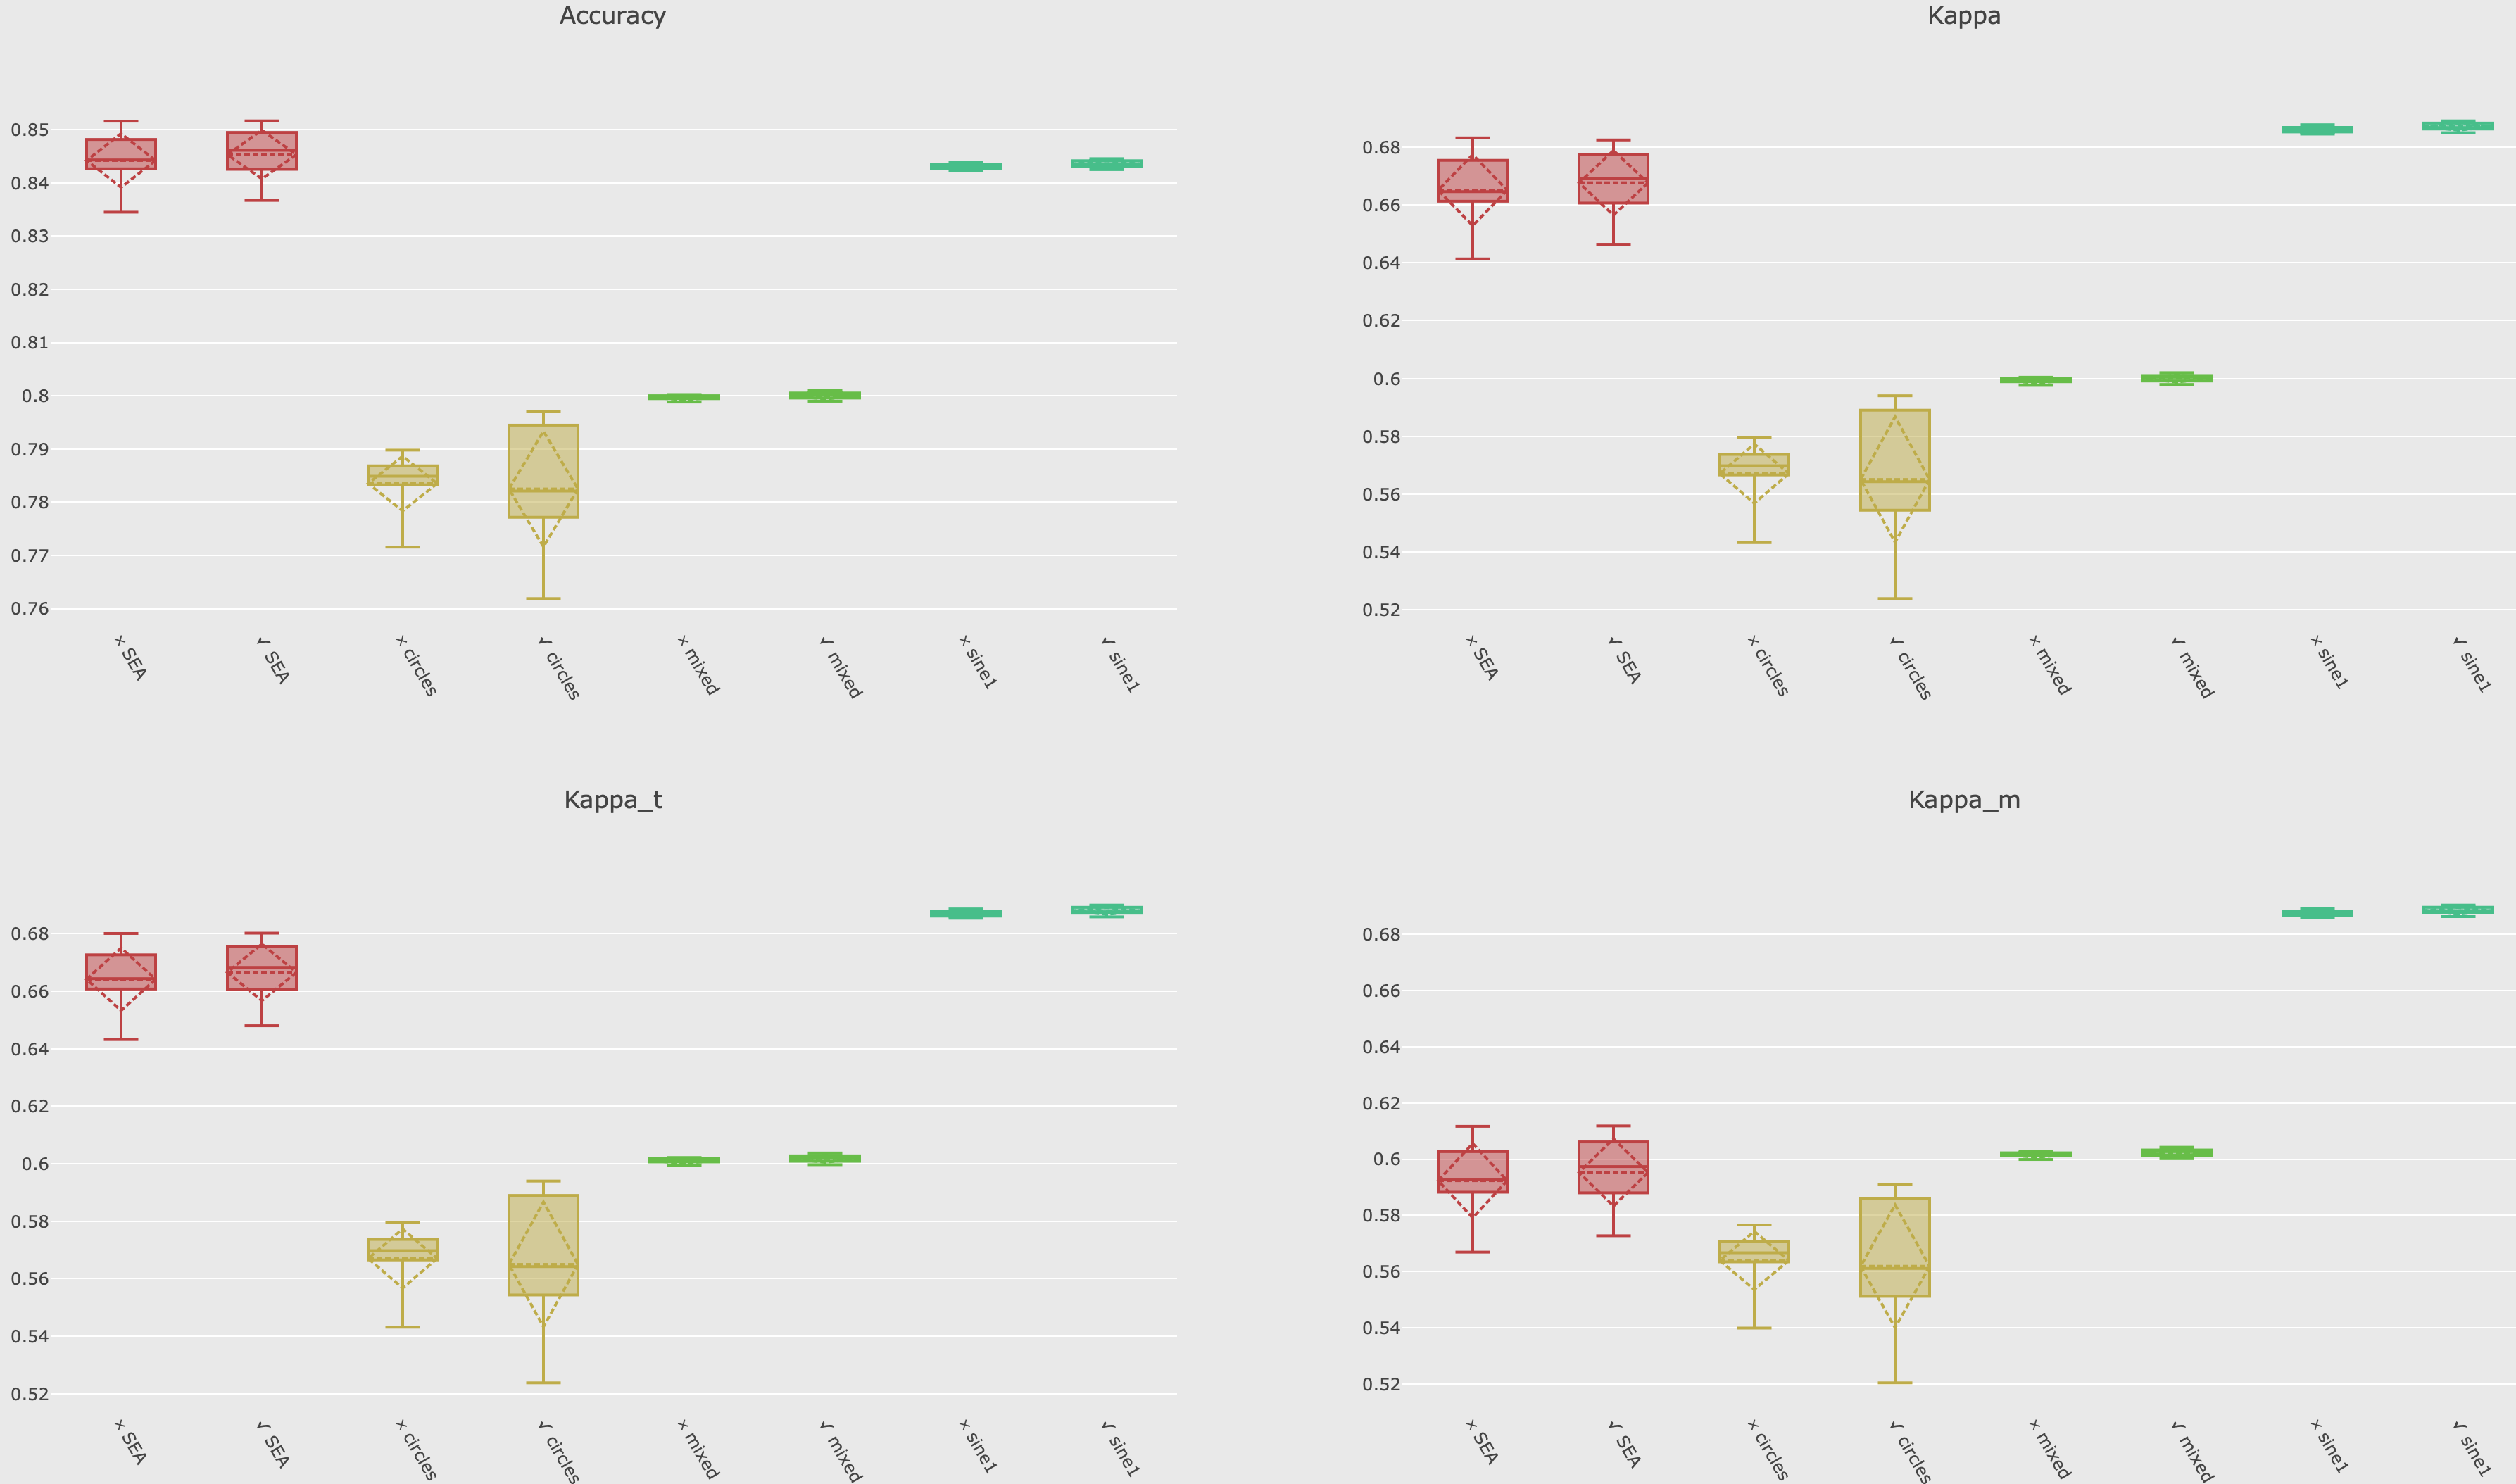
\includegraphics[width=\linewidth]{./images/boxplot_params_use_w}
\caption{\label{fig:boxplot_params_use_w}Boxplots showing performance over 4 datasets (using un/weighted probabilities for drift detection)}
\end{figure}

Our modified drift detectors using the probabilities will be called MFHDDM/S (M for modified).
Algorithm \ref{alg:pfhddm} shows the implementation for MFHDDM. MFHDDMS is different from MFHDDM only in that it keeps track of an additional shorter sliding window. No changes were necessary to implement FHDDM/S with the different boolean, as Dr. Pesaranghader's currently works with boolean values.

\begin{algorithm}
\caption{Modified Fast Hoeffding Drift Detection Method (MFHDDM)\label{alg:pfhddm}}
\Fn{init(window\_size, delta, use\_probability)}{
    (n, $\delta$, p) = (window\_size, delta, use\_probability)\;
    $\epsilon_d = \sqrt{\frac{1}{2n}ln\frac{1}{\delta}}$\;
    reset()\;
}

\Fn{reset()}{
    w=[]\;
    $\mu^m=0$\;
}

\Fn{detect(p)}{
    \If{w.size = n}{
        w.tail.drop()\;
    }
    w.push(p)\;
    \eIf{$w.size < n$}{
        return False\;
    }{
        \eIf{use\_probability}{
            $\mu^t=w.average()$\;
        }{
            $\mu^t=\frac{w.count(True)}{w.size()}$\;
        }
        \If{$\mu^m < \mu^t$}{
            $\mu^m =\mu^t$\;
        }
        $\Delta\mu = \mu^m - \mu^t$\;
        \eIf{$\Delta\mu \ge \epsilon_d$}{
            reset()\;
            \Return True\;
        }{
            \Return False\;
        }
    }
}
\end{algorithm}

%----------------------------------------------------------------------------------------

\section{A toy example}

In this section, we will explain how an instance from the stream is processed from beginning to end. The reader should refer to algorithm \ref{alg:pipeline_pseudocode} and figure \ref{fig:not_yet_uploaded}.

The first step in the algorithm is pre-training the algorithm so that it can start with a decent model of the data. Therefore a parameter is used to dictate the number of instances that the ensemble is to train on before starting the interleaved test-then-train loop, where the entirety of the work of this thesis takes part in.

Next, the interleaved test-then-train loop begins. For this toy example, we will use a batch size of one. In this batch (or chunk), there will be a single instance, which we will refer to as $X$, and its true class value which will be referred to as $y$.

The ensemble will first be tasked with predicting the class value, denoted $\hat{y}$, of $X$. In order to do so, the ensemble will require each classifier it contains to assign a probability that $X$ belongs to a class, for each possible value that the class can take. For example, in the case of a binary classification problem, $y \in [0,1]$. So in our example, each classifier needs to predict $P(X, y=0)$, and $P(X, y=1)$ given its model of the data. The ensemble will then keep a copy of these predictions and apply a weighting function to the original values. The weighting function, as previously stated, reduces values in $[0,0.7[$ and increases values in $]0.7, 1]$. Finally, the ensemble will average the probabilities for each class class value (again, for binary classification). It will do the same for the weighted probabilities. The ensemble will now have four values: $p_0, p_1 = \frac{1}{n}\sum_{i=1}^{n} P_i(X, y=Y)\ \forall\ Y$,  $w_0,w_1=\frac{1}{n}\sum_{i=1}^{n} w(P_i(X, y=Y))\ \forall\ Y$, where $n$ is the number of classifiers in the ensemble, $w(x)$ is the weighting function seen in section \ref{section:new_voting_strategy}, $P_i(X, y=0)$ is the probability that classifier $i$ assigns $X$ to class $0$. $Y$ is the set of possible class values.
The maximum of $p_0$ and $p_1$ will determine the class the ensemble predicts for $X$. If $p_0$ is the maximum value, then $\hat{y}=0$, and in the opposite case where $p_1$ is the maximum value then $\hat{y}=1$.

The next step in the interleaved test-then-train loop is dedicated to drift detection. When drifts are detected, we want to keep a sliding window of the previously seen instances (the size of this window is the same as the window size used for the training step) for retraining the classifiers. In order to detect drifts, a modified version of FHDDMS is used. The average probability for the winning class, which we mentioned earlier as being copied, is passed to the drift detector. Until the sliding windows within the drift detector are full, the detector will not run. There are two sliding windows: one short to detect abrupt drifts, and a longer one to detect gradual concept drifts. The sliding window will, therefore, keep track, as discussed in section \ref{section:new_voting_strategy}, of either the probabilities or the boolean indicating whether a classifier predicted the "winning" vote. In the case of the probabilities, the Hoeffding bound is used to detect if the average probability drifts too far from the maximum seen average probability. In the case of the boolean values, a drift is detected, using the Hoeffding bound again, when the classifier in question predicts less often on average according to the "winning" vote.
When a drift is detected, the drift detector's windows are emptied, the classifiers in the ensemble are either all reset or a subset of them are reset. 
If a drift is detected, the sliding window of previously seen instances is then used to retrain all of the classifiers in the ensemble.

If no drift is detected, there is a chance (set by a parameter) that the $y$ value (the real class value of $X$) will be replaced by $\hat y$ (the predicted class value of $X$).

The final step in the interleaved test-then-train loop is to train the ensemble on the $<X, y>$ tuple. In order to do so, a hybrid sliding-tumbling window (as seen in section \ref{section:hybrid-windows}) is used within the ensemble to train the classifiers contained, again, within it. In this case, since $<X, y>$ is the first instance seen by the ensemble during the interleaved test-then-train loop (as in this is the first iteration of the prequential evaluation loop) it is added to the hybrid window. This hybrid window has a size of the batch size (in this case 1) times the number of classifiers in the ensemble (in this case let us say 3). 
Only one classifier in the ensemble is trained on the hybrid window's tuples. In order to do so, an index is kept inside the ensemble. This index points to the classifier to train and is incremented at each $ensemble.train()$ call, and a modulus is applied on the index to keep it within the range of classifiers in the ensemble.
So classifier $c_0$ is selected to train on the hybrid window, containing a single tuple at the moment.

At this point, the first iteration of the interleaved test-then-train loop has terminated, and the framework computes the global metrics required (accuracy, kappa statistics, etc) as well as over a sliding window of the last 200 instances.

\begin{algorithm}
\caption{Data processing pipeline\label{alg:pipeline_pseudocode}}
\Fn{evaluate\_prequential(ensemble, pretrain\_size, batch\_size, window\_size)}{
    ensemble.train(pretrain\_size)\;
    window = fifo\_queue(size = window\_size)\;
    \While{stream.has\_more\_samples()}{
        X, y = stream.next\_sample(batch\_size)\;
        window.add([X,y])\;

        prediction, probabilities, weighted\_probabilities = ensemble.test(X)\;
        
        drift\_detected = drift\_detection(prediction\ \textbf{or}\ probabilities\ \textbf{or}\ weighted\_probabilities)\;

        \If{random() > ground\_truth\_percentage \textbf{and}\ not\ drift\_detected}{
            replace\_y(y, prediction)\;
        }
        
        \If{drift\_detected}{
            ensemble.reset(window)\;
        }
        
        ensemble.train(X, y)\;
    }
}

\Fn{ensemble.train(X, y)}{
    \tcp{instance variables $clfs$ stores the classifiers in ensemble \& $mod$ stores the current index 
    of the classifier to train}
    ensemble.clfs[ensemble.mod].train(X, y)\;
    ensemble.mod = (ensemble.mod + 1) modulus (length(ensemble.clfs))\;
}

\Fn{ensemble.test(X)}{
    p, w\_p = [], []\;
    \For{$classifier \in ensemble.classifiers$}{
        prob = classifier.predict()\;
        p.add(prob), w\_p.add([weight(prob[0]), weight(prob[1]))\;
    }
    \tcp{map subclassifier probabilities to single probability}
    avg, w\_avg = p.avg(), w\_p.avg()\;
    prediction = class\_of\_max(w\_avg)\;
    \Return prediction, avg, w\_avg\;
}

\Fn{weight(prediction\_probability)}{
    \Return $\frac{1-tanh(3.5-7\times prediction\_probability)}{2}$\;
}

\Fn{drift\_detection(value, use\_probability)}{
    window.push(value)\;
    \If{$window.size > max\_window\_size$}{
        window.tail.drop()\;
        \eIf{use\_probability}{
            $\mu^t=window.average()$\;
        }{
            $\mu^t=\frac{window.count(True)}{window.size()}$\;
        }
        \If{$\mu^m < \mu^t$}{
            $\mu^m =\mu^t$\;
        }
        $\Delta\mu = \mu^m - \mu^t$\;
        \If{$\Delta\mu \ge \epsilon\_d$}{
            \Return True\ \textbf{and} reset();
        }
    }
    \Return False\;
}
\end{algorithm}

%----------------------------------------------------------------------------------------

\section{Summary}
Over the course of this chapter, we have introduced our RGTDSMF methodology. The first was to propose a new weighting function for our ensemble classifier. The second was a novel windowing technique for classifiers within an ensemble that delays their training. The third was investigating how implementing our ensemble to self-train on a portion of the training data could influence its performance. The fourth and final contribution was to extend FHDDM/S to operate without any knowledge of the ground truth. We have described the components of our methodology and their algorithms.